\documentclass[10pt,a4paper]{article}
\usepackage[T1]{fontenc}
\usepackage[utf8]{inputenc}
\usepackage{lmodern}
\usepackage[margin=25mm]{geometry}
\usepackage{amsmath,amssymb,booktabs,graphicx}
\usepackage{caption,float,needspace}
\usepackage[hidelinks]{hyperref}
\captionsetup{font=small}
\setlength{\parindent}{0pt}
\setlength{\parskip}{5pt}
\setlength{\emergencystretch}{2em}
\newcommand{\ind}{\mathbf{1}}
\hypersetup{pdftitle={Bootstrap uncertainty in sidewalk-hazard rankings}}
\begin{document}
\section*{Bootstrap uncertainty in sidewalk-hazard rankings}

We evaluate whether uncertainty from repeated classifier fits improves the ranking of sidewalk images for hazard review. We focus on the binary hazard task with a fixed review budget of 46 images. We compare three methods: penalizing probability uncertainty, summarizing rank distributions, and finding a consensus from pairwise outranking. We compare these to two baselines: the original single DINO model and the unadjusted mean of the bootstrap heads.

\section{Training independent heads with bootstrapping}
\label{sec:training}
The ensemble uses the previously chosen Pittsburgh-only configuration. A frozen DINOv3 ViT-B/16 backbone maps each RGB $224\times224$ image (with ImageNet normalization) to a 768-dimensional CLS feature vector $z_i$. We train $B=128$ separate linear hazard heads, each producing
\begin{equation}
p_i^{(b)}=\operatorname{sigmoid}\!\left(w_b^{\mathsf T}z_i+c_b\right),
\qquad b=1,\ldots,B.
\end{equation}
The backbone is shared and fixed, and we do not use training images from other cities.

The training set contains 1,276 records (527 hazards and 749 non-hazards). To keep exact image duplicates together, we group records by their RGB pixel hash, yielding 1,236 groups (including 40 duplicate pairs). We stratify these groups based on their ratio of hazards to non-hazards. For each head, we bootstrap sample the groups within each stratum, keeping all records from the sampled groups. Each head therefore receives 1,276 records with the original class balance, but the specific records vary. The samples contain an average of 807.3 distinct records.

Each head uses different random seeds for bootstrapping, initialization, and batch shuffling. We train using Adam with a learning rate of $3\times10^{-5}$, weight decay of $0.01$, batch size of 64, and 5,000 parameter updates to minimize unweighted binary cross-entropy. We keep the final checkpoint for all 128 heads without validation-based early stopping. This yields 128 aligned hazard probabilities per observation.

Our first baseline is the original single head, trained on the full Pittsburgh split without bootstrapping. Its predictions are used directly. The second baseline is the simple average of the 128 bootstrap predictions. We evaluate all methods on the same images and labels.

\section{Uncertainty-adjusted probability ranking}
\label{sec:adjusted}
For observation $i$, we define the ensemble mean and sample standard deviation as:
\begin{equation}
\mu_i=\frac{1}{B}\sum_{b=1}^{B}p_i^{(b)},\qquad
s_i=\sqrt{\frac{1}{B-1}\sum_{b=1}^{B}\left(p_i^{(b)}-\mu_i\right)^2}.
\end{equation}
The standard ranking simply orders images by their mean score $\mu_i$. To penalize uncertain predictions across the fitted heads, we define an adjusted score:
\begin{equation}
S_i(\lambda)=\mu_i-\lambda s_i.
\end{equation}
Here, $s_i$ measures variability across heads, not the standard error of the mean. Scores are not clipped to $[0,1]$, and exact ties are broken using ascending sample IDs.

We tune $\lambda$ using validation precision@46 over a grid from 0 to 4, selecting the smallest value if there are ties. We also test a conservative baseline: the 5th percentile of the 128 probabilities. Both methods favor stable predictions, though neither guarantees a higher true-hazard yield at a fixed budget. The standard deviation penalty explicitly trades off high average probability for cross-head stability.

\section{Rank distributions and selection frequencies}
\label{sec:ranks}
Instead of adjusting probabilities, we can measure uncertainty in the rankings directly. For each head, we rank all images by hazard probability (rank 1 is highest, ties get midranks). Let $r_i^{(b)}$ be this rank. We report the expected rank $\overline r_i$ and the 95\% midrank interval $I_i$:
\begin{equation}
\overline r_i=\frac{1}{B}\sum_b r_i^{(b)},\qquad
I_i=\left[Q_{0.025}(r_i^{(1:B)}),Q_{0.975}(r_i^{(1:B)})\right].
\end{equation}
This interval captures rank variation across refits without adding random tie-breaking noise.

We also track how often an image appears in the top $k$. Let $a_i^{(b)}$ be the number of images ranked strictly above $i$, and $t_i^{(b)}$ be the number tied with $i$. Allocating tied slots equally, the frequency of appearing in the top $k$ is:
\begin{equation}
\widehat P_k(i)=\frac{1}{B}\sum_b
\min\!\left\{1,\max\!\left\{0,\frac{k-a_i^{(b)}}{t_i^{(b)}}\right\}\right\}.
\end{equation}
We evaluate two new orderings: increasing expected rank $\overline r_i$ and decreasing top-46 frequency $\widehat P_{46}(i)$. Neither ordering uses true hazard labels. The expected-rank ordering is equivalent to weighted Borda aggregation.

\section{Pairwise outranking and consensus}
\label{sec:pairwise}
For each pair of images, we calculate how often one outranks the other across the heads:
\begin{equation}
W_{ij}=\frac{1}{B}\sum_b\ind[p_i^{(b)}>p_j^{(b)}],\qquad
T_{ij}=\frac{1}{B}\sum_b\ind[p_i^{(b)}=p_j^{(b)}].
\end{equation}
This preserves the dependence between predictions. A pairwise consensus seeks a final ranking $\pi$ that maximizes agreement with these pairwise probabilities. Writing $C_{ij}=BW_{ij}$, the Kemeny objective is:
\begin{equation}
\pi^*\in\operatorname*{arg\,max}_{\pi}
\sum_{1\leq a<b\leq N}C_{\pi(a),\pi(b)}.
\label{eq:objective}
\end{equation}
This objective differs from both expected rank and true-hazard yield. Since majority preferences may form cycles, we first decompose the majority graph into strongly connected components. Within each component, we use a binary integer program to find a valid linear ordering, adding transitivity constraints iteratively:
\begin{equation}
0\leq x_{ij}+x_{jk}-x_{ik}\leq1,\qquad i<j<k.
\end{equation}
The optimizer only sees probabilities, not true hazard labels.

\section{Results}
\label{sec:results}
\subsection{Validation comparison}
We rank all 382 validation images (157 hazards) with a budget of $k=46$ (12.04\% of the split). For ordering $\pi$ and hazard indicator $y_i$, we define:
\begin{equation}
\operatorname{Precision@46}=\frac{\sum_{a=1}^{46}y_{\pi(a)}}{46},\qquad
\operatorname{Recall@46}=\frac{\sum_{a=1}^{46}y_{\pi(a)}}{\sum_i y_i}.
\end{equation}
Precision@46 is our primary metric. Tuning the standard deviation penalty $\lambda$ yields a maximum of 34 hazards for grid values between 0 and 0.35. Our tie-breaking rule selects $\lambda=0$, meaning the penalized score reduces exactly to the unadjusted mean. The 5th-percentile method finds 32 hazards. All other methods (original head, mean, expected rank, top-46 frequency, and pairwise consensus) tie at 34 hazards (Table~\ref{tab:validation}).
\begin{table}[H]
\centering
\caption{Validation comparison on 382 images, including 157 hazards. Precision and recall are percentages. $^{\dagger}$The original model is selected by the parsimony tie-break described below.}
\label{tab:validation}
\small
\begin{tabular}{lrrr}
\toprule
Ranking & Hazards & Precision@46 & Recall@46 \\
\midrule
Original single head (no bootstrap)$^{\dagger}$ & 34/46 & 73.91 & 21.66 \\
Unadjusted mean (128 heads) & 34/46 & 73.91 & 21.66 \\
Mean minus SD penalty ($\lambda=0$) & 34/46 & 73.91 & 21.66 \\
Fifth probability percentile & 32/46 & 69.57 & 20.38 \\
Expected rank (Borda) & 34/46 & 73.91 & 21.66 \\
Top-46 selection frequency & 34/46 & 73.91 & 21.66 \\
Pairwise consensus (Kemeny) & 34/46 & 73.91 & 21.66 \\
\bottomrule
\end{tabular}
\end{table}
\begin{figure}[H]
\centering
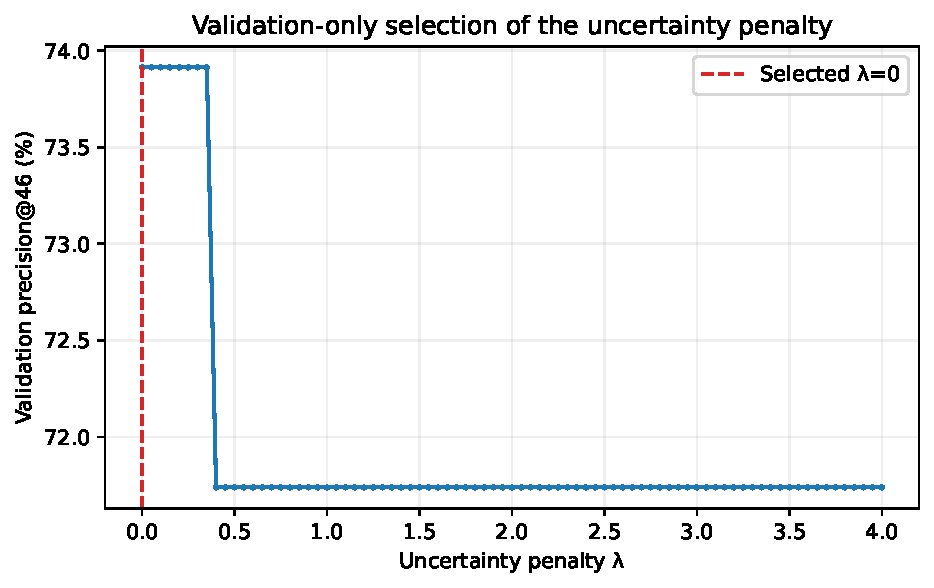
\includegraphics[width=.76\linewidth]{figures/point_2_validation_lambda_sweep.pdf}
\caption{Validation-only tuning of the SD penalty. The smallest maximizing value is $\lambda=0$; no test scores enter this sweep.}
\label{fig:lambda}
\end{figure}

\Needspace{14\baselineskip}
\subsection{Selection between the two reference rankings}
\label{sec:selection}
Since the original single head and the 128-head mean both achieve 73.91\% validation precision, the uncertainty-aware methods provide no strict advantage. We resolve the tie using parsimony: we select the original single DINO head because it requires only one head instead of 128.

\textbf{We select the original single DINO head without bootstrapping.} This is a simplicity tie-break, not proof that the original model is more accurate. The following test results reflect this choice.

\subsection{Test performance after selection}
\label{sec:test}
The test split has 380 images (174 hazards). Table~\ref{tab:test} shows the performance of all methods using a 46-image budget.
\begin{table}[H]
\centering
\caption{Test comparison after the validation-based selection, on 380 images including 174 hazards. $^{\dagger}$Previously selected original model; the selection is not changed using this table.}
\label{tab:test}
\small
\begin{tabular}{lrrr}
\toprule
Ranking & Hazards & Precision@46 & Recall@46 \\
\midrule
Original single head (no bootstrap)$^{\dagger}$ & 26/46 & 56.52 & 14.94 \\
Unadjusted mean (128 heads) & 27/46 & 58.70 & 15.52 \\
Mean minus SD penalty ($\lambda=0$) & 27/46 & 58.70 & 15.52 \\
Fifth probability percentile & 26/46 & 56.52 & 14.94 \\
Expected rank (Borda) & 27/46 & 58.70 & 15.52 \\
Top-46 selection frequency & 28/46 & 60.87 & 16.09 \\
Pairwise consensus (Kemeny) & 27/46 & 58.70 & 15.52 \\
\bottomrule
\end{tabular}
\end{table}

The original single head retrieves 26 test hazards. The mean, SD-penalty ($\lambda=0$), expected rank, and pairwise consensus all retrieve 27. The top-46 frequency retrieves 28. While the ensemble mean and frequency rankings find 1-2 more hazards than the single head, this minor difference does not establish statistical superiority or justify overturning our validation-based choice.

\subsection{What the uncertainty analyses reveal}
Even when methods retrieve the same number of hazards, individual image rankings can vary wildly. Table~\ref{tab:stability} shows that the typical rank interval spans over 150 positions. Only 14 images are consistently placed in the top 46. Notably, about half of these highly stable selections are non-hazards---demonstrating that the ensemble can be confidently wrong.
\begin{table}[H]
\centering
\caption{Rank stability across 128 heads. Interval widths are in rank positions; other quantities are counts of images.}
\label{tab:stability}
\small
\begin{tabular}{lrr}
\toprule
Statistic & Validation & Test \\
\midrule
Median rank-interval width & 156.2 & 162.2 \\
90th-percentile interval width & 208.4 & 215.8 \\
Intervals crossing rank 46 & 100 & 112 \\
Images with $\widehat P_{46}\geq0.95$ & 14 & 14 \\
Hazards among these stable selections & 9 & 8 \\
Non-hazards among these stable selections & 5 & 6 \\
Images with $\widehat P_{46}>0$ & 158 & 171 \\
\bottomrule
\end{tabular}
\end{table}

The pairwise consensus achieves a certified global optimum (Table~\ref{tab:optimality}). While it changes over 270 positions compared to the expected-rank ordering, the top-46 sets are almost identical. This highlights that optimizing global pairwise agreement does not necessarily improve a strict top-k review objective.
\begin{table}[H]
\centering
\caption{Pairwise optimization certificates. Objectives count head-pair agreements, not true hazards.}
\label{tab:optimality}
\small
\begin{tabular}{lrrrr}
\toprule
Split & Feasible objective & Upper bound & Gap & Optimal \\
\midrule
Validation & 8,235,639 & 8,235,639 & 0 & Yes \\
Test & 8,102,338 & 8,102,338 & 0 & Yes \\
\bottomrule
\end{tabular}
\end{table}

Ultimately, while uncertainty summaries are useful for exposing unstable predictions, none of the uncertainty-aware rankings significantly improved top-46 precision over the baseline models. The single original head remains our chosen model based on parsimony, though the ensemble is still valuable for generating rank intervals and pairwise comparisons alongside that decision.

\clearpage
\subsection{Rank intervals and pairwise heatmaps}
\begin{figure}[H]
\centering
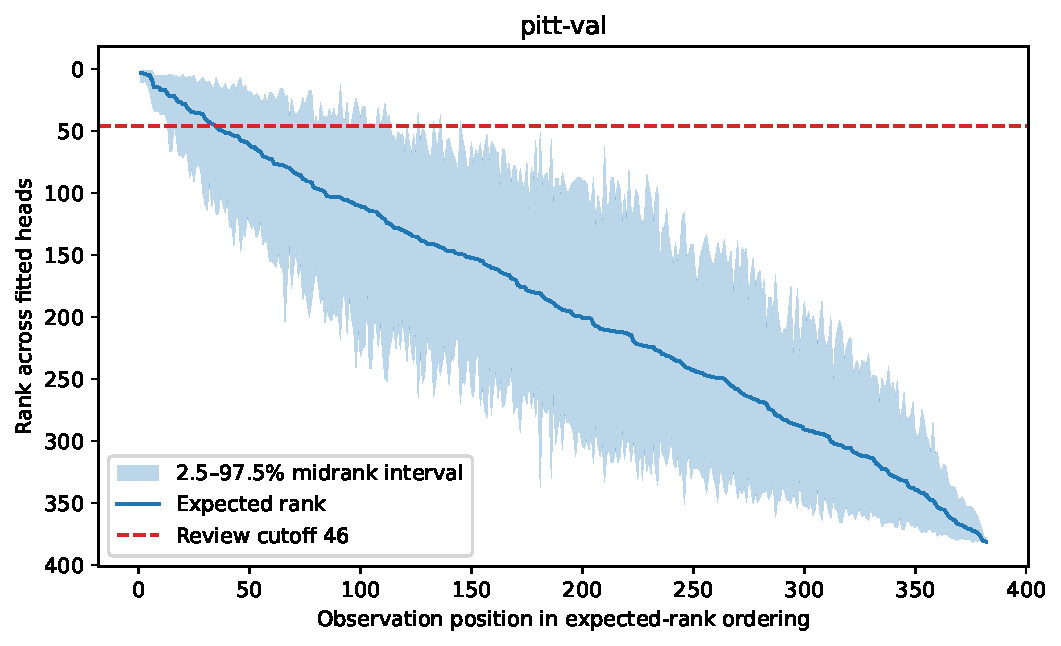
\includegraphics[width=.88\linewidth]{figures/point_3_pitt-val_rank_intervals.pdf}
\caption{Validation rank intervals. Images are ordered by expected rank; shading is the 2.5th--97.5th percentile interval and the dashed line marks rank 46.}
\label{fig:val-intervals}
\end{figure}
\begin{figure}[H]
\centering
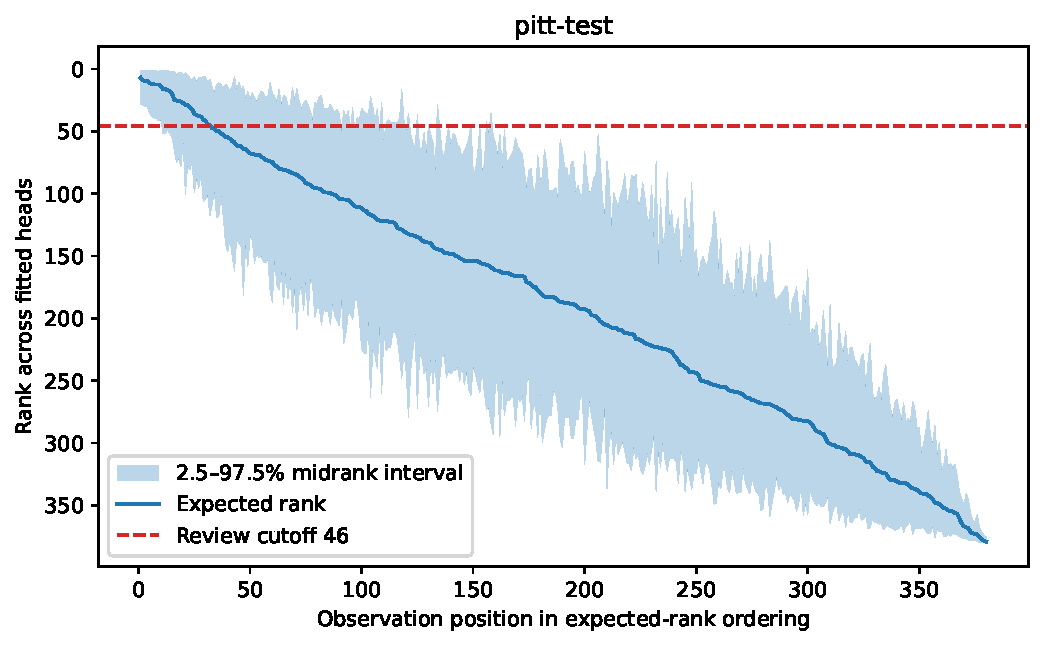
\includegraphics[width=.88\linewidth]{figures/point_3_pitt-test_rank_intervals.pdf}
\caption{Test rank intervals, reported after the selection. Lower ranks indicate higher review priority.}
\label{fig:test-intervals}
\end{figure}
\clearpage
\begin{figure}[H]
\centering
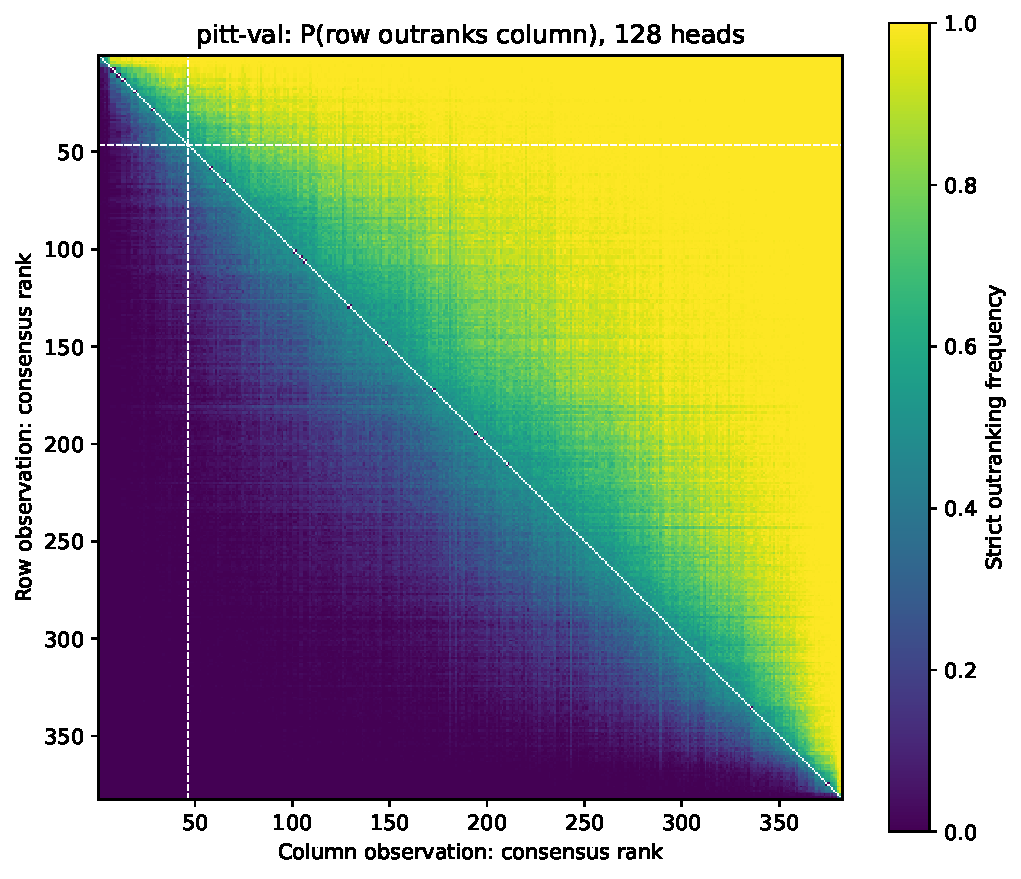
\includegraphics[width=.68\linewidth]{figures/point_4_pitt-val_pairwise_heatmap.pdf}
\caption{Validation strict outranking frequencies $W_{ij}$ in consensus order. A cell is the fraction of heads in which its row image outranks its column image; dashed lines mark the top-46 boundary.}
\label{fig:val-heatmap}
\end{figure}
\begin{figure}[H]
\centering
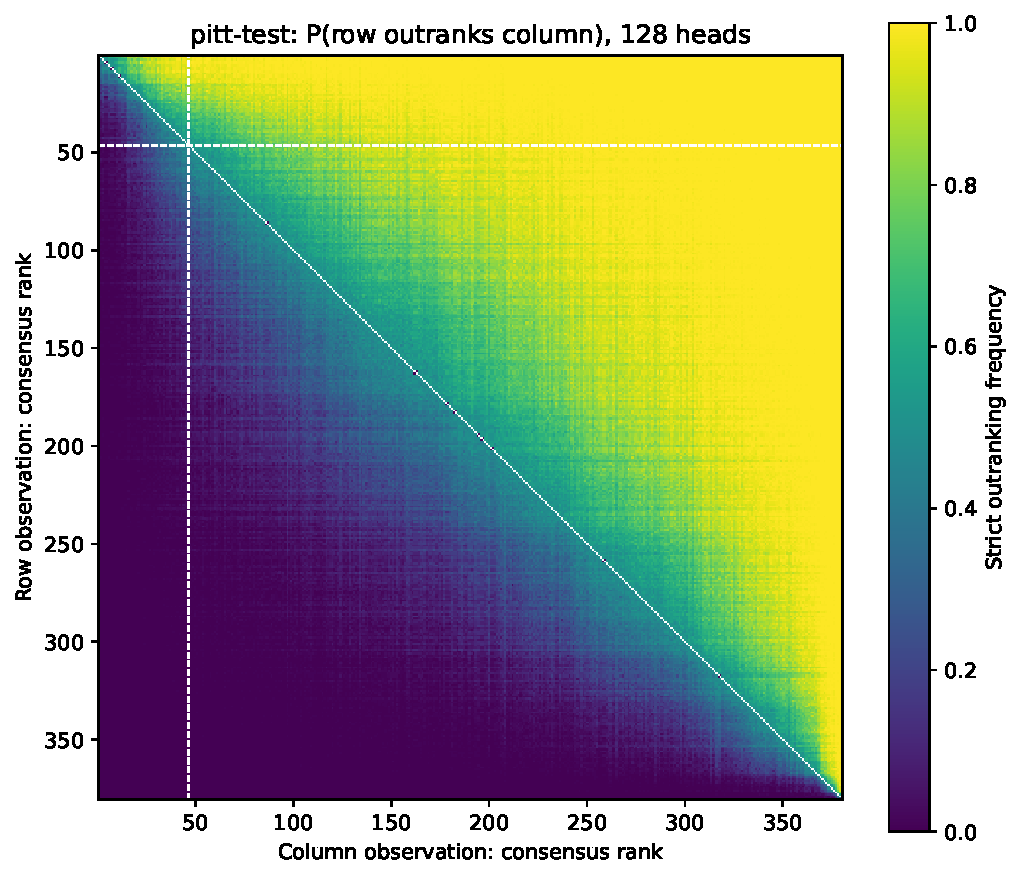
\includegraphics[width=.68\linewidth]{figures/point_4_pitt-test_pairwise_heatmap.pdf}
\caption{Test strict outranking frequencies, reported after selection, on the same $[0,1]$ scale. The diagonal is masked. Exact score ties are represented separately and are not forced to probability 0.5 in this matrix.}
\label{fig:test-heatmap}
\end{figure}
\end{document}
